%# -*- coding:utf-8 -*-
%%%%%%%%%%%%%%%%%%%%%%%%%%%%%%%%%%%%%%%%%%%%%%%%%%%%%%%%%%%%%%%%%%%%%%%%%%%%%%%%%%%%%

\pagecolor{titlegray}\afterpage{\pagecolor{white}\printwatermark}

\noindent{\fzcuyasongc\zihao{4}\ziju{.15}中国科学院指定考研参考书}
\vfill
\begin{center}
{\maokai\zihao{0}\ziju{.5}線性代數}
\vfill\fzqiti\zihao{4}
李炯生\hspace{1\ccwd}查建国\rlap{\hspace*{.8\ccwd}{\normalsize\fzxian{}编著}}
\vfill
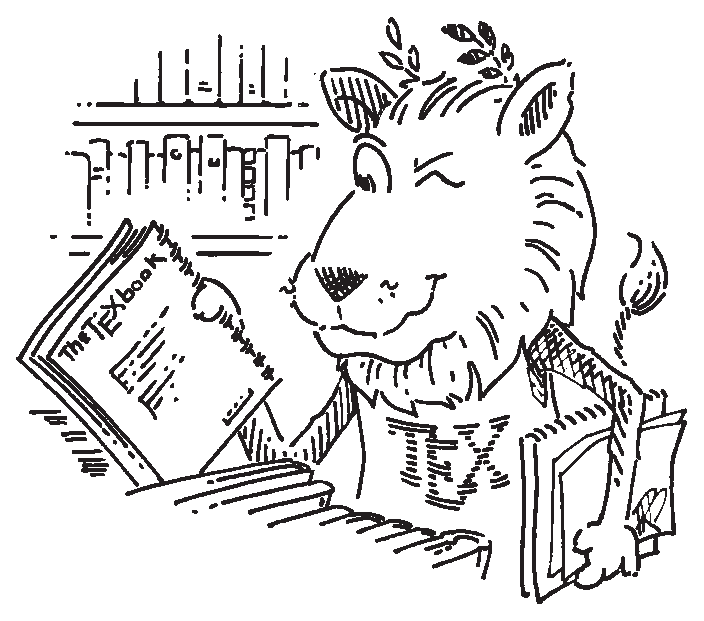
\includegraphics[width={.6\linewidth}]{ctanlion.eps}
\vfill\vspace*{-1cm}\fzfangguo\ziju{0.2}\zihao{-3}
中国科学技术大学出版社\\[1mm]
\TeXGyreBonum\normalsize\textbf{1~9~8~9}
\end{center}

\clearpage

\chapter*{\zihao{4}\fzydzhhei\ziju{1}内容提要}

\begin{changemargin}{8mm}{8mm}
\newbox\CIPInf
\sbox\CIPInf{\parbox[c]{.75\linewidth}{\parindent\ccwd
线性代数~/~李炯生,查建国编著.{}—合肥:中国科学技术大学出版社,1989\,(2005.9~重印,2010.10~重排)\par
(中国科学院指定考研参考书)\par
{\ttfamily\bfseries ISBN 978-7-312-00110-9}
\par\medskip
I. 线…\enskip{} II. \DingNum{1}~李…~~\DingNum{2}~查…\enskip{} III. 线性代数—高等学校—教材\enskip{} IV. O\,151.2
\par\medskip
中国版本图书馆~CIP~数据核字(2003)第~078690~号}}
\newbox\COPYRIGHT
\sbox\COPYRIGHT{\parbox[c]{.75\linewidth}{\parindent\ccwd\bfseries\fzsonghei\CMRoman
《线性代数》版权归中国科学技术大学出版社所有,本重排本仅限用于个人学习和~\XeLaTeX~排版技术交流,请勿用于任何
商业行为,因私自散布造成的法律及相关问题,重排者一律不予负责!本书已有第二版发行,全国各大书店均应有售,请支持、购买正版!}}
\newbox\TeXlion
\sbox\TeXlion{
\includegraphics[width={.1\linewidth}]{tex-lion.pdf}}
\newbox\GNULogo
\sbox\GNULogo{
\includegraphics[width={.15\linewidth}]{gnulogo.eps}}

\fzwkai\TeXGyreBonum

本书是作者在中国科学技术大学数学系多年教学的基础上编写而成的.它由多项式、行列式、矩阵、线性空间、线性变
换、Jordan~标准形、Euclid~空间、酉空间和双线性函数等九章组成.在内容的叙述上,力图做到矩阵方法与几何方法
并重.每章都配有丰富的典型例题和充足的习题可供读者选用.

附录中收录龚昇教授编著的《线性代数五讲》,从现代数学,尤其是模论的观点来重新审视与认识线性代数,讨论了向
量空间、线性变换,着重研究了主理想整环上的模及其分解,并以此来重新理解向量空间在线性算子作用下的分解,可
以使读者从高一个层次上来认识线性代数.

本书适合作为综合性大学理科数学专业的教材,也可以作为各类大专院校师生的教学参考书,以及关心线性代数与矩阵
论的科技工作者和数学爱好者的自学读物或参考书.

\centering

\vspace{\stretch{4}}

\noindent\begin{tabu}{m{.75\linewidth}X[mc]}
\multicolumn{2}{l}{\kern\ccwd\emph*{图书在版编目~\textsf{(CIP)}~数据}}  \\
\specialrule{1pt}{1pt}{5pt}
\usebox\CIPInf                 &   \usebox\GNULogo     \\
\specialrule{1pt}{5pt}{0pt}
\end{tabu}

\vspace{\stretch{4}}

\noindent\begin{tabu}{m{.75\linewidth}@{}X[mc]}
\multicolumn{2}{l}{\fzxbsong\zihao{-4}\ziju{.5}郑重声明}   \\
\specialrule{1pt}{1pt}{5pt}
\usebox\COPYRIGHT              &   \usebox\TeXlion     \\
\specialrule{1pt}{5pt}{5pt}
\end{tabu}

\noindent\normalsize\emph*{版权归原出版社所有\hspace{.8\ccwd}侵权必究}\hfill\mbox{}
\end{changemargin}
